\documentclass{standalone}
\usepackage{tikz}
\usepackage{tikz-qtree}
\usetikzlibrary{backgrounds, fit}

\begin{document}
  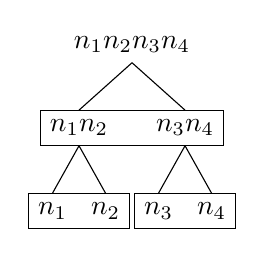
\begin{tikzpicture}
	\Tree [.\node (1234) {$n_1n_2n_3n_4$};
	  [.\node (12) {$n_1n_2$};
		[.\node (1) {$n_1$}; ] 
		[.\node (2) {$n_2$}; ]] 
	  [.\node (34) {$n_3n_4$};
		[.\node (3) {$n_3$}; ] 
		[.\node (4) {$n_4$}; ]]]

	\begin{pgfonlayer}{background}
	  \node () [rectangle, draw, fit = (1) (2), inner sep = 0pt] {};
	  \node () [rectangle, draw, fit = (3) (4), inner sep = 0pt] {};
	  \node () [rectangle, draw, fit = (12) (34), inner sep = 0pt] {};
	\end{pgfonlayer}
  \end{tikzpicture}
\end{document}
